\section{Medições em laboratório}

Montaremos os dois circuitos discutidos anteriormente em laboratório e mediremos a tensão de saída em seis configurações de formato de onda e frequências diferentes. Esses parâmetros serão definidos por um dispositivo Arduino com $11$ saídas, cada uma com tensão esperada de $5V$.

\begin{figure}[H]
    \centering
    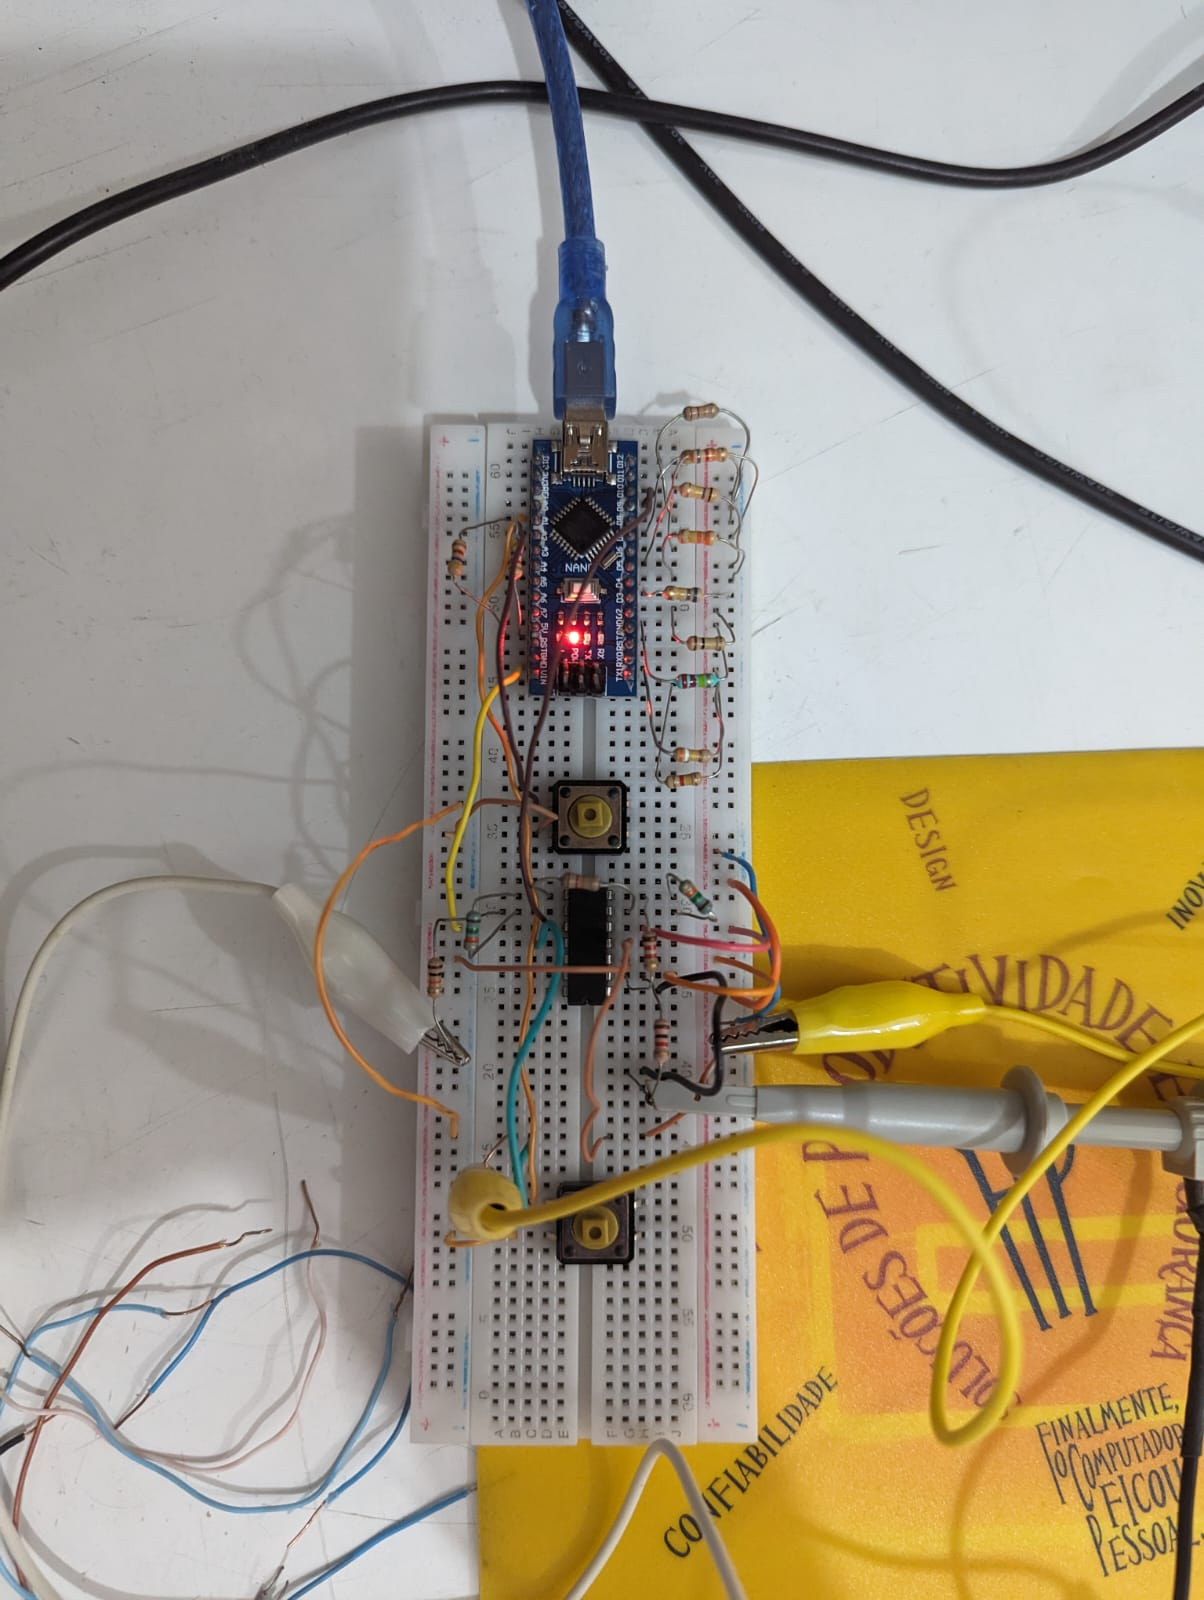
\includegraphics[width=0.35\columnwidth]{images/circuito_montado.jpeg}
    \caption{Vista superior do circuito montado em laboratório.}
\end{figure}

\begin{figure}[H]
    \centering
    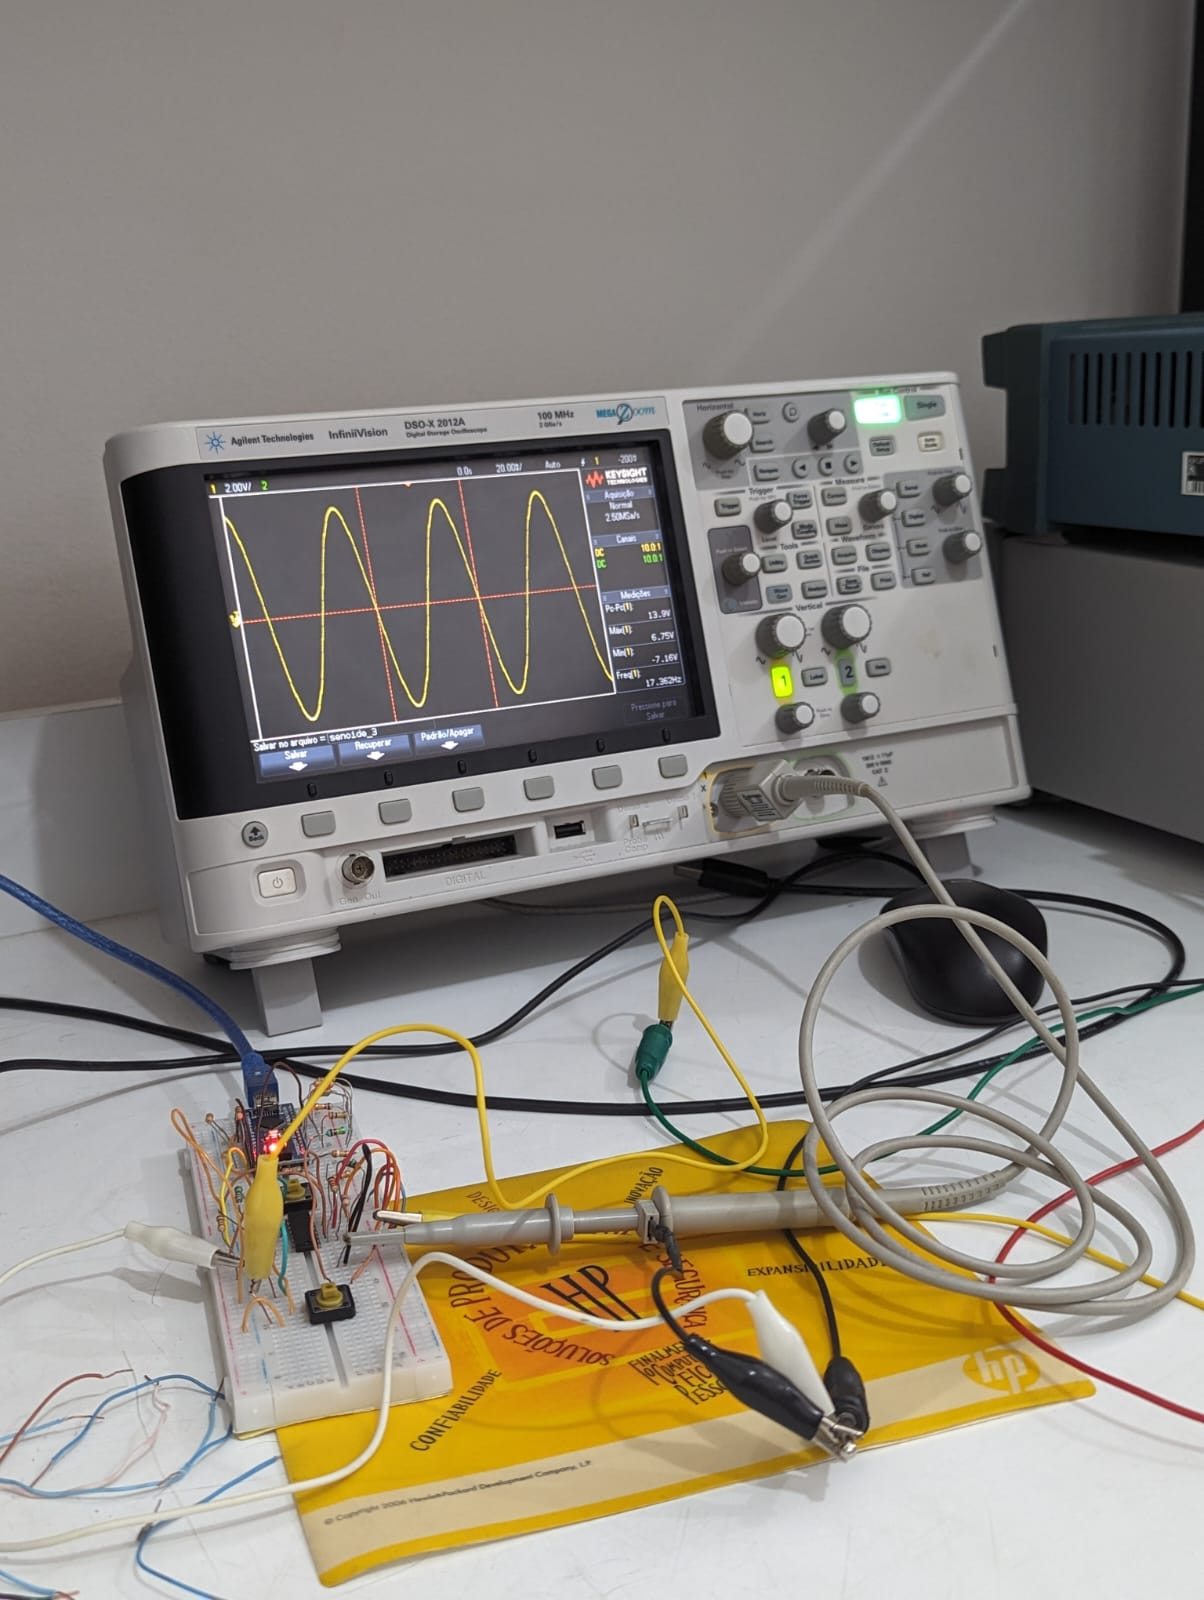
\includegraphics[width=0.35\columnwidth]{images/circuito_e_osciloscopio.jpeg}
    \caption{Circuito montado em laboratório e osciloscopio.}
\end{figure}

\newpage

\subsection{Componentes}

Com os valores calculados na secao anterior, tenta-se utilizar componentes comerciais com valores compativeis com os calculados. Os componentes utilizados sao:

\begin{figure}[H]
    \centering
    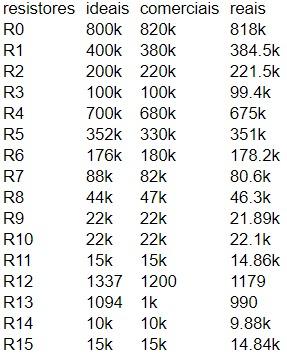
\includegraphics[width=0.35\columnwidth]{images/tabela_componentes.jpeg}
    \caption{Tabela de componentes utilizados.}
\end{figure}

\subsection{Configuração Senoidal}

Medimos três frequências diferentes de configuração Senoidal, e são estas as seguintes:

\begin{figure}[H]
    \centering
    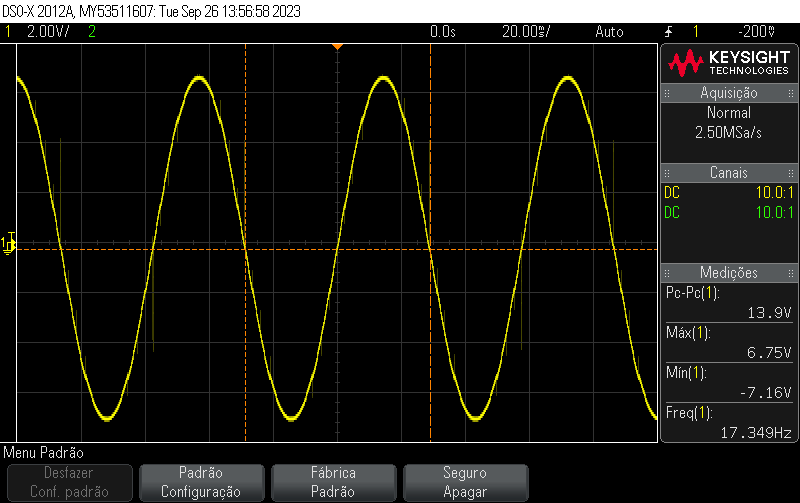
\includegraphics[width=0.5\columnwidth]{images/senoide_2.png}
    \caption{Onda de saída senoidal com frequência de $17.35Hz$.}
\end{figure}

\begin{equation}
    \begin{aligned}
         & V_{pp} = 13.9 V    \\
         & V_{max} = 6.75 V   \\
         & V_{min} =  -7.16 V \\
         & Freq = 17.35 Hz
    \end{aligned}
\end{equation}

\begin{figure}[H]
    \centering
    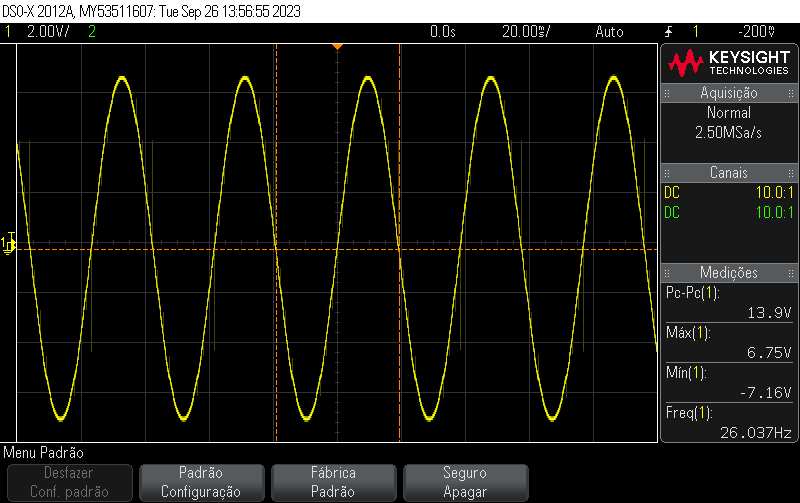
\includegraphics[width=0.5\columnwidth]{images/senoide_1.png}
    \caption{Onda de saída senoidal com frequência de $26.03Hz$.}
\end{figure}

\begin{equation}
    \begin{aligned}
         & V_{pp} = 13.9 V    \\
         & V_{max} = 6.75 V   \\
         & V_{min} =  -7.16 V \\
         & Freq = 26.037 Hz
    \end{aligned}
\end{equation}

\begin{figure}[H]
    \centering
    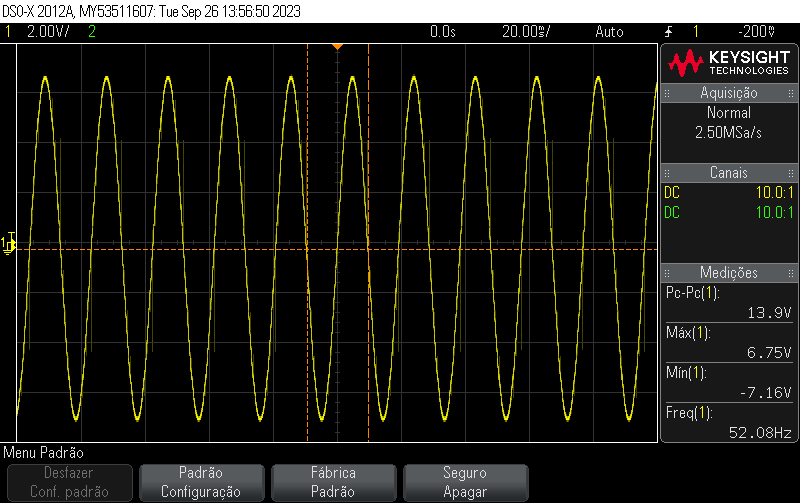
\includegraphics[width=0.5\columnwidth]{images/senoide_0.png}
    \caption{Onda de saída senoidal com frequência de $52.08Hz$.}
\end{figure}

\begin{equation}
    \begin{aligned}
         & V_{pp} = 13.9 V    \\
         & V_{max} = 6.75 V   \\
         & V_{min} =  -7.16 V \\
         & Freq = 52.08 Hz
    \end{aligned}
\end{equation}

\newpage

\subsection{Configuração Triangular}

Medimos três frequências diferentes de configuração Triangular, e são estas as seguintes:

\begin{figure}[H]
    \centering
    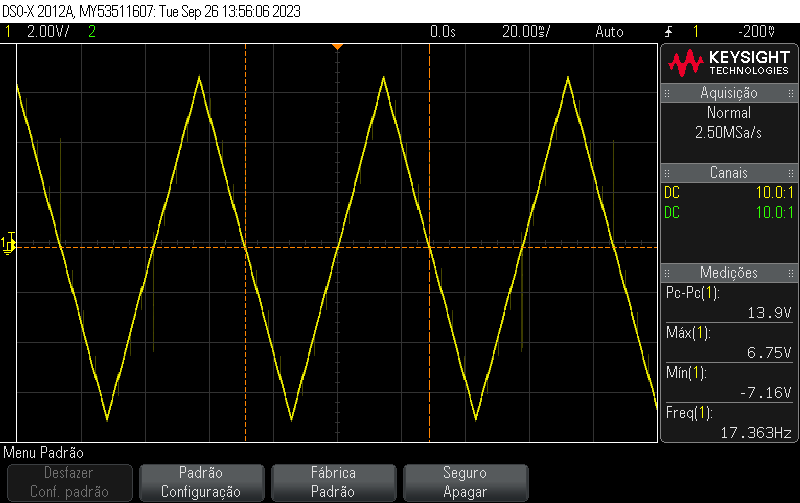
\includegraphics[width=0.5\columnwidth]{images/triangular_2.png}
    \caption{Onda de saída triangular com frequência de $17.363Hz$.}
\end{figure}

\begin{equation}
    \begin{aligned}
         & V_{pp} = 13.9 V    \\
         & V_{max} = 6.75 V   \\
         & V_{min} =  -7.16 V \\
         & Freq = 17.35 Hz
    \end{aligned}
\end{equation}

\begin{figure}[H]
    \centering
    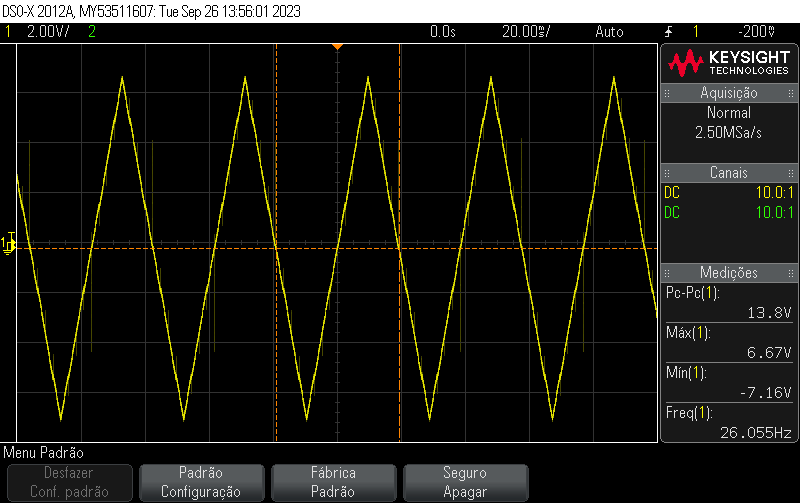
\includegraphics[width=0.5\columnwidth]{images/triangular_1.png}
    \caption{Onda de saída triangular com frequência de $26.055Hz$.}
\end{figure}

\begin{equation}
    \begin{aligned}
         & V_{pp} = 13.8 V    \\
         & V_{max} = 6.67 V   \\
         & V_{min} =  -7.16 V \\
         & Freq = 26.055 Hz
    \end{aligned}
\end{equation}

\begin{figure}[H]
    \centering
    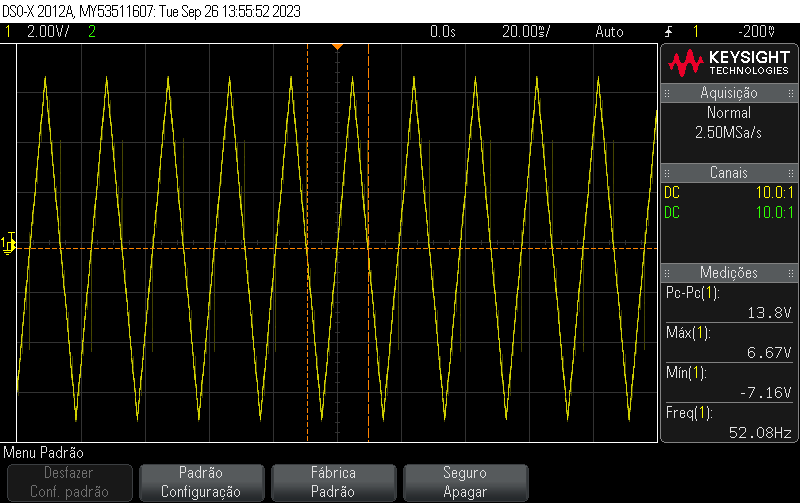
\includegraphics[width=0.5\columnwidth]{images/triangular_0.png}
    \caption{Onda de saída triangular com frequência de $52.08Hz$.}
\end{figure}

\begin{equation}
    \begin{aligned}
         & V_{pp} = 13.8 V    \\
         & V_{max} = 6.67 V   \\
         & V_{min} =  -7.16 V \\
         & Freq = 52.08 Hz
    \end{aligned}
\end{equation}

\subsection{Tensão de saída do Arduino}

Nesta imagem, analisamos o $V_m$ que o Arduino pode fornecer em cada um dos seus pinos de saída, que na fundamentação teórica assumimos que seria de $5V$.

\begin{figure}[H]
    \centering
    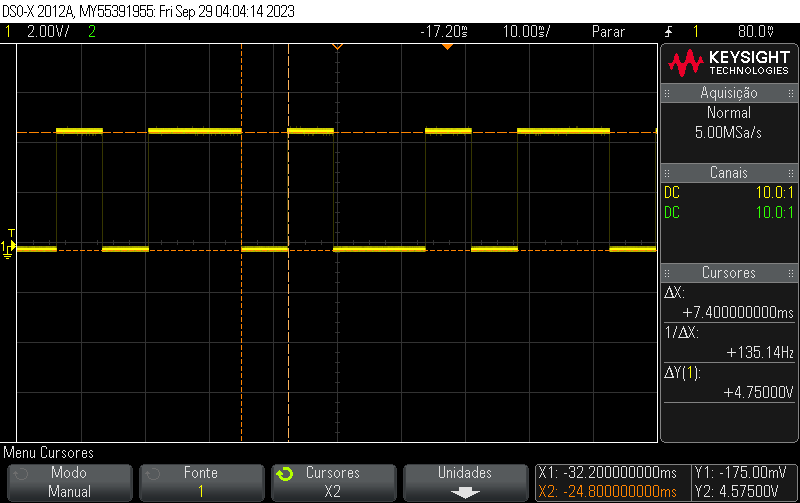
\includegraphics[width=0.5\columnwidth]{images/VM_segundo_laboratorio.png}
    \caption{Tensão do pino de saída do Arduino.}
\end{figure}

Observa-se que o pino de saída do Arduino tem tensão de $4,75V$, e não $5V$ como o esperado.

\newpage
